% Basierend auf der TEX-Vorlage "Briefvorlage für Privatleute"
% Von Alexey Abel
% Orginal-Git-Repository: https://github.com/PanCakeConnaisseur/latex-briefvorlage-din-5008
% Basiert auf KOMA-Scripts scrlttr2

\documentclass[
	% Schriftgröße
	fontsize=12pt,
	%
	% zwischen Absätzen eine leere Zeile einfügen, statt lediglich Einrückung
	parskip=full,
	%
	% Papierformat auf DIN-A4
	paper=A4,	
	%
	% Briefkopf (ganz oben) rechts ausrichten, standardmäßig links
	fromalign=right,
	%
	% Telefonnummer im Briefkopf anzeigen
	%fromphone=true,
	%
	% Faxnnummer im Briefkopf anzeigen
	%fromfax=true,
	%
	% E-Mail-Adresse im Briefkopf anzeigen
	fromemail=true,
	%
	% URL im Briefkopf anzeigen
	%fromurl=true,
	%
	% Faltmarkierungen verbergen
	%foldmarks=false,
	%
	% Die neuste Version von scrlettr2 verwenden 
	version=last,
]{scrlttr2}

% Zeichenkodierung des Dokuments ist in UTF-8
\usepackage[utf8]{inputenc}

% Sprache des Dokuments auf Deutsch
\usepackage[ngerman]{babel}

% Includen von PDFs nach dem Brief, siehe \includepdf unten
\usepackage{pdfpages}

% klickbare Links und E-Mail-Adressen. Paket url kann keine klickbaren,
% deswegen hyperref. Option hidelinks versteckt farbigen Rahmen.
\usepackage[hidelinks]{hyperref}



\begin{document}

% Name nach Schlussgruß (unter Unterschrift) nicht nach rechts einrücken
\renewcommand*{\raggedsignature}{\raggedright}



% Absendername
\setkomavar{fromname}{Paul Goldschmidt}

% Absenderadresse
\setkomavar{fromaddress}{69123 Heidelberg}

% Absenderfax
% (oben fromfax=true setzen)
%\setkomavar{fromfax}{+49 222 222 22}

% Absender-E-Mail-Adresse
% der erste Paremeter ist fürs Klicken, der zweite wird angezeigt/gedruckt
\setkomavar{fromemail}{\href{mailto:kontakt@paul-goldschmidt.de}{kontakt@paul-goldschmidt.de}}


% Ort beim Datum
\setkomavar{place}{Heidelberg}

% Datum
\setkomavar{date}{\today}

% Betreff
\setkomavar{subject}{Unterstützung bei einem offenen Brief an Frau Dr. Eisenmann in der Sache des COVID-19-Umgangs an Schulen}



% Kundennummer
%\setkomavar{customer}[\customername]{DE-112233}

% Ihr Zeichen
%\setkomavar{yourref}[\yourrefname]{IZ-12345}

% Ihr Schreiben vom
%\setkomavar{yourmail}[\yourmailname]{1. April 2018}



\begin{letter}{
	Lehrerinnen und Lehrer\\
	sowie Schülerinnen und Schüler\\
	des Bundeslandes\\
	Baden-Württemberg
}

\opening{Sehr geehrte Lehrkräfte, liebe Mitschüler*innen,}

letzten Donnerstag gab die Kultusministerin unseres Bundeslandes, Frau Dr. Susanne Eisenmann zu Protokoll, \glqq [dass] Präsenz\-unterricht an Schulen als oberstes Ziel [gesehen wird]\grqq{}\footnote{Quelle: Rhein-Neckar-Zeitung, 22.10.2020: \href{https://www.rnz.de/politik/suedwest_artikel,-baden-wuerttemberg-eisenmann-sieht-praesenzunterricht-an-schulen-als-oberstes-ziel-update-_arid,568110.html}{\color{blue}Eisenmann sieht Präsenzunterricht an Schulen als oberstes Ziel (Update)}, abgerufen am 31.10.2020, 10:30 Uhr}. Ich als Schüler kann jedoch den Wunsch des Kultusministeriums, Schulen unbedingt offen zu halten, nicht nachvollziehen. Und das ging nicht nur mir so: In meiner Position als SMV-Vorstandsmitglied der Carl-Bosch-Schule Heidelberg und als Jugendgemeinderat der Stadt Heidelberg wurde vielfach an mich die Bitte herangetragen, den Schulleitungen der Region Alternativsysteme zum dauerhaften und mit allen Klassen gleichzeitigem Präsenz\-unterricht vorzuschlagen. Doch die Schulleitungen können selbst nicht handeln, da sie Anweisungen des Kultusministeriums gebunden sind. Sinnvolle Alternativen wie das rollierende System, in dem Klassen beispielsweise nur jede zweite Woche Präsenz\-unterricht haben, haben sich schon letztes Schuljahr zwischen den Pfingstferien und den Sommerferien bewährt. Diese Alternative wird vom Kultusministerium nicht in Betracht gezogen.

Deshalb habe ich mich entschlossen, die Anregungen von Schü\-ler*innen sowie von Lehrer*innen in einem offenen Brief an Frau Dr. Eisenmann darzulegen, mit dem Ziel, ein Umdenken im Kultusministerium anzuregen.\\Und dafür brauche ich Ihre Hilfe: Wenn Sie ebenfalls mit der aktuellen Handhabung der COVID-19-Situation an den Schulen Unzufrieden sind, und diese gerne Verbessern würden bitte ich Sie und euch, den offenen Brief an Frau Dr. Eisenmann mit zu unterzeichnen. Dieser lässt sich \href{https://raw.githubusercontent.com/PaulGoldschmidt/offener-brief-eisenmann/main/Brief_Eisenmann/brief.pdf}{\color{blue}unter diesem Link im Internet\footnote{\href{https://github.com/PaulGoldschmidt/offener-brief-eisenmann}{github.com/PaulGoldschmidt/offener-brief-eisenmann}}} oder an die Mail angehängt finden. Ein offener Brief gewinnt mit jeder Unterzeichnung an Nachdrücklichkeit. 
Wenn Sie/Ihr den Brief unterzeichnen wollen, geht das folgendermaßen: Bitte schreiben Sie eine kurze Mail von Ihrem Schulmailaccount\footnote{So kann nachvollzogen werden, dass Sie eine Verbindung zu der Schule haben - sollte Ihre Schule keine offiziellen Mailaccounts besitzen, so bitte ich um eine Mail an {\href{mailto:brief@paul-goldschmidt.de}{brief@paul-goldschmidt.de}, damit eine Lösung gefunden werden kann.}} mit Ihrem Namen, Ihrer Position (Lehrer, Schüler oder sonstige Positionen in Verbindung mit der Schule), dem Schulnamen und einem (Datenschutz-)Einverständnis, dass diese Informationen im Rahmen des offenen Briefes veröffentlicht werden dürfen. Die Informationen zum Datenschutz sind auf den nächsten Seiten dieses Dokumentes zu finden. 
Eine Mail zum Unterzeichnen des Briefes könnte wie folgt aussehen: \\\\
\noindent\rule{\textwidth}{0.5pt}
\textsf{Hallo,\\\\hiermit unterzeichne ich, VORNAME NACHNAME, den offenen Brief an Frau Dr. Eisenmann. Ich bin LEHRKRAFT/SCHÜLER*IN auf der SCHULNAME. Ich bin mit der Veröffentlichung meines Namens, der Rolle (Lehrkraft/Schüler*in) und dem dazugehörigen Schulnamen einverstanden und habe die Datenschutzerklärung zur Kenntnis genommen und willige dieser ein.\\}
\noindent\rule{\textwidth}{0.5pt}
\\\\Bitte senden Sie eine Mail mit eben beschriebenem Inhalt an \href{mailto:brief@paul-goldschmidt.de}{\color{blue}brief@paul-goldschmidt.de}, damit ich Sie in die Unterschriftenliste einfügen kann. \\
Sie müssen sich keine Sorgen machen, eventuell alleine auf der Unterschriftenliste zu stehen: Der Brief wird überhaupt erst veröffentlicht, wenn 150 Unterschriften gesammelt wurden, und auch auf keinen Fall vor Donnerstag, dem 5. November 2020. Damit wird gewährleistet, dass alle genug Zeit zum Unterschreiben haben. \\
Ich freue mich über jede Teilnahme.
\closing{Vielen Dank und bleiben Sie gesund!}

% Anlage(n)
% Standardmäßig wird "Anlage(n)" eingefügt, dies kann überschrieben werden, hier mit "Anlagen"
\encl{Datenschutzerklärung, Unterschriftenliste für Schulen}

% Verteiler
%\cc{Bürgermeister, Vereinsvorsitzender}

\end{letter}

% Weitere PDFs können automatisch angefügt werden, z.B. Ahnänge.
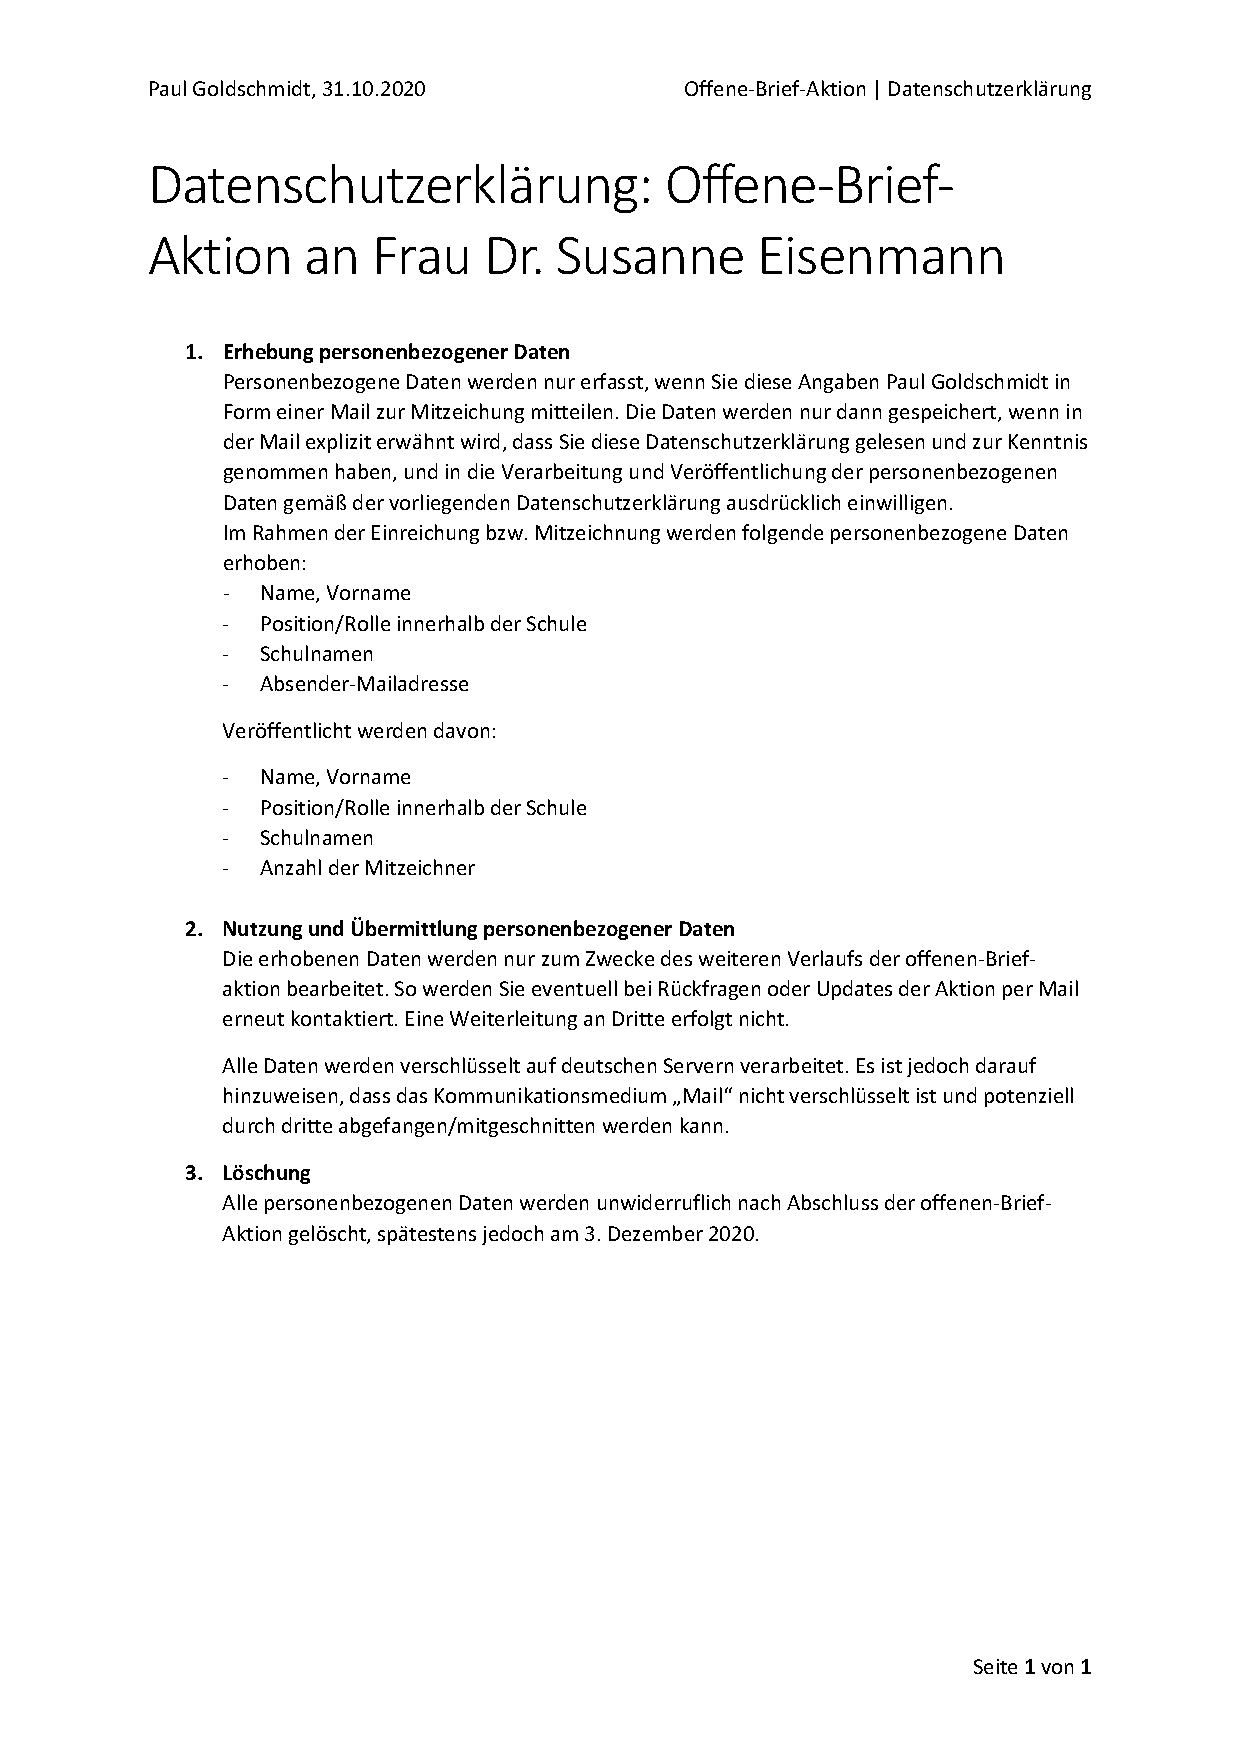
\includepdf[pages=-]{Datenschutzerklaerung.pdf}
% Pfad ist relativ zu dieser tex-Datei. Mit .. ein Verzeichnis hoch.
% Der pages-Parameter spezifiziert welche Seiten eingefügt werden.
% Beispiele:
% pages=-				alle Seiten
% pages={1-4}			Seite 1-4
% pages={1,4,5}			Seite 1, 4 und 5
% pages={3,{},8-11,15}	Seite 3, leere Seite, Seite 8-11 und Seite 15
% Der openright-Parameter startet die Anlagen auf ungerader (rechter) Seite, d.h. notfalls wird eine leere Seite
% eingefügt. Im doppelseitigem Druck wird dadurch besser zwischen Brief und Anlage getrennt. Für einseitigen Druck
% entfernen.

\end{document}
